% !TEX TS-program = pdflatexmk
\documentclass{./packages/optica-article}
\graphicspath{{images/}{practica1/images}}
\journal{opticajournal}

\usepackage{csvsimple}
\usepackage{siunitx}
\usepackage{physics}
\usepackage{booktabs}
\usepackage{tikz}

\usepackage{caption}
\usepackage{subcaption}
\usetikzlibrary{positioning}

\newcommand{\sinc}{\textrm{sinc}}
\newcommand\conv{\circledast}

% Set the article type
\articletype{Research Article}
\begin{document}

\title{Caracterización de sistemas de formación de imágenes}

\author{Adriana Mamani Lazarte\authormark{1} Alex G. Recuenco\authormark{1}, y Carlos España Castaño\authormark{1}}

\address{\authormark{1}Universidad Complutense de Madrid, Madrid, CP 28040, España}

\section{Introducción}
En esta práctica vamos a caracterizar un sistema de formación de imágenes mediante la determinación experimental de su función de transferencia de modulación (MTF). Para ello utilizaremos un método directo (el test de barras) y un método indirecto (el test de borde). La MTF nos aportará información sobre el rango de frecuencias espaciales, estimar su resolución y el contraste de la imagen a estudiar.

Para tal fin anteriormente mencionado tuvimos que entender la respuesta a un impulso, la función de transferencia de modulación de la imagen, el poder distinguir si nuestro sistema es lineal e invariante con respecto a su desplazamiento y sus descripciones.

\section{Marco práctico}
El sistema cuya MTF mediremos consiste en un objetivo de microscopio con apertura numérica $\textrm{NA} = 0,25$ y un aumento $10\times$ (F10),
y una cámara CCD con un tamaño de píxel de $s=4,65 \unit{\micro\meter}$.
Las imágenes captadas por la cámara se visualizarán en la pantalla del PC.
A continuación se detallará el procedimiento práctico realizado utilizando los dos métodos de medición de la MTF.

\subsection{Medida de MTF mediante el test de barras (método directo)}\label{sec:metodo-directo}

Se utilizó el test USAF 1951 (Fig.~\ref{fig:usaf1951}) como imagen general en la que se captaron fotografías de  distintos elementos de rendijas de la diapositiva de la Fig.~\ref{fig:usafpic} presentada a continuación. Se controla la exposición para obtener los colores grises en cada muestra de imagen sin sobre-exposición.

\begin{figure}[h]
	\centering
	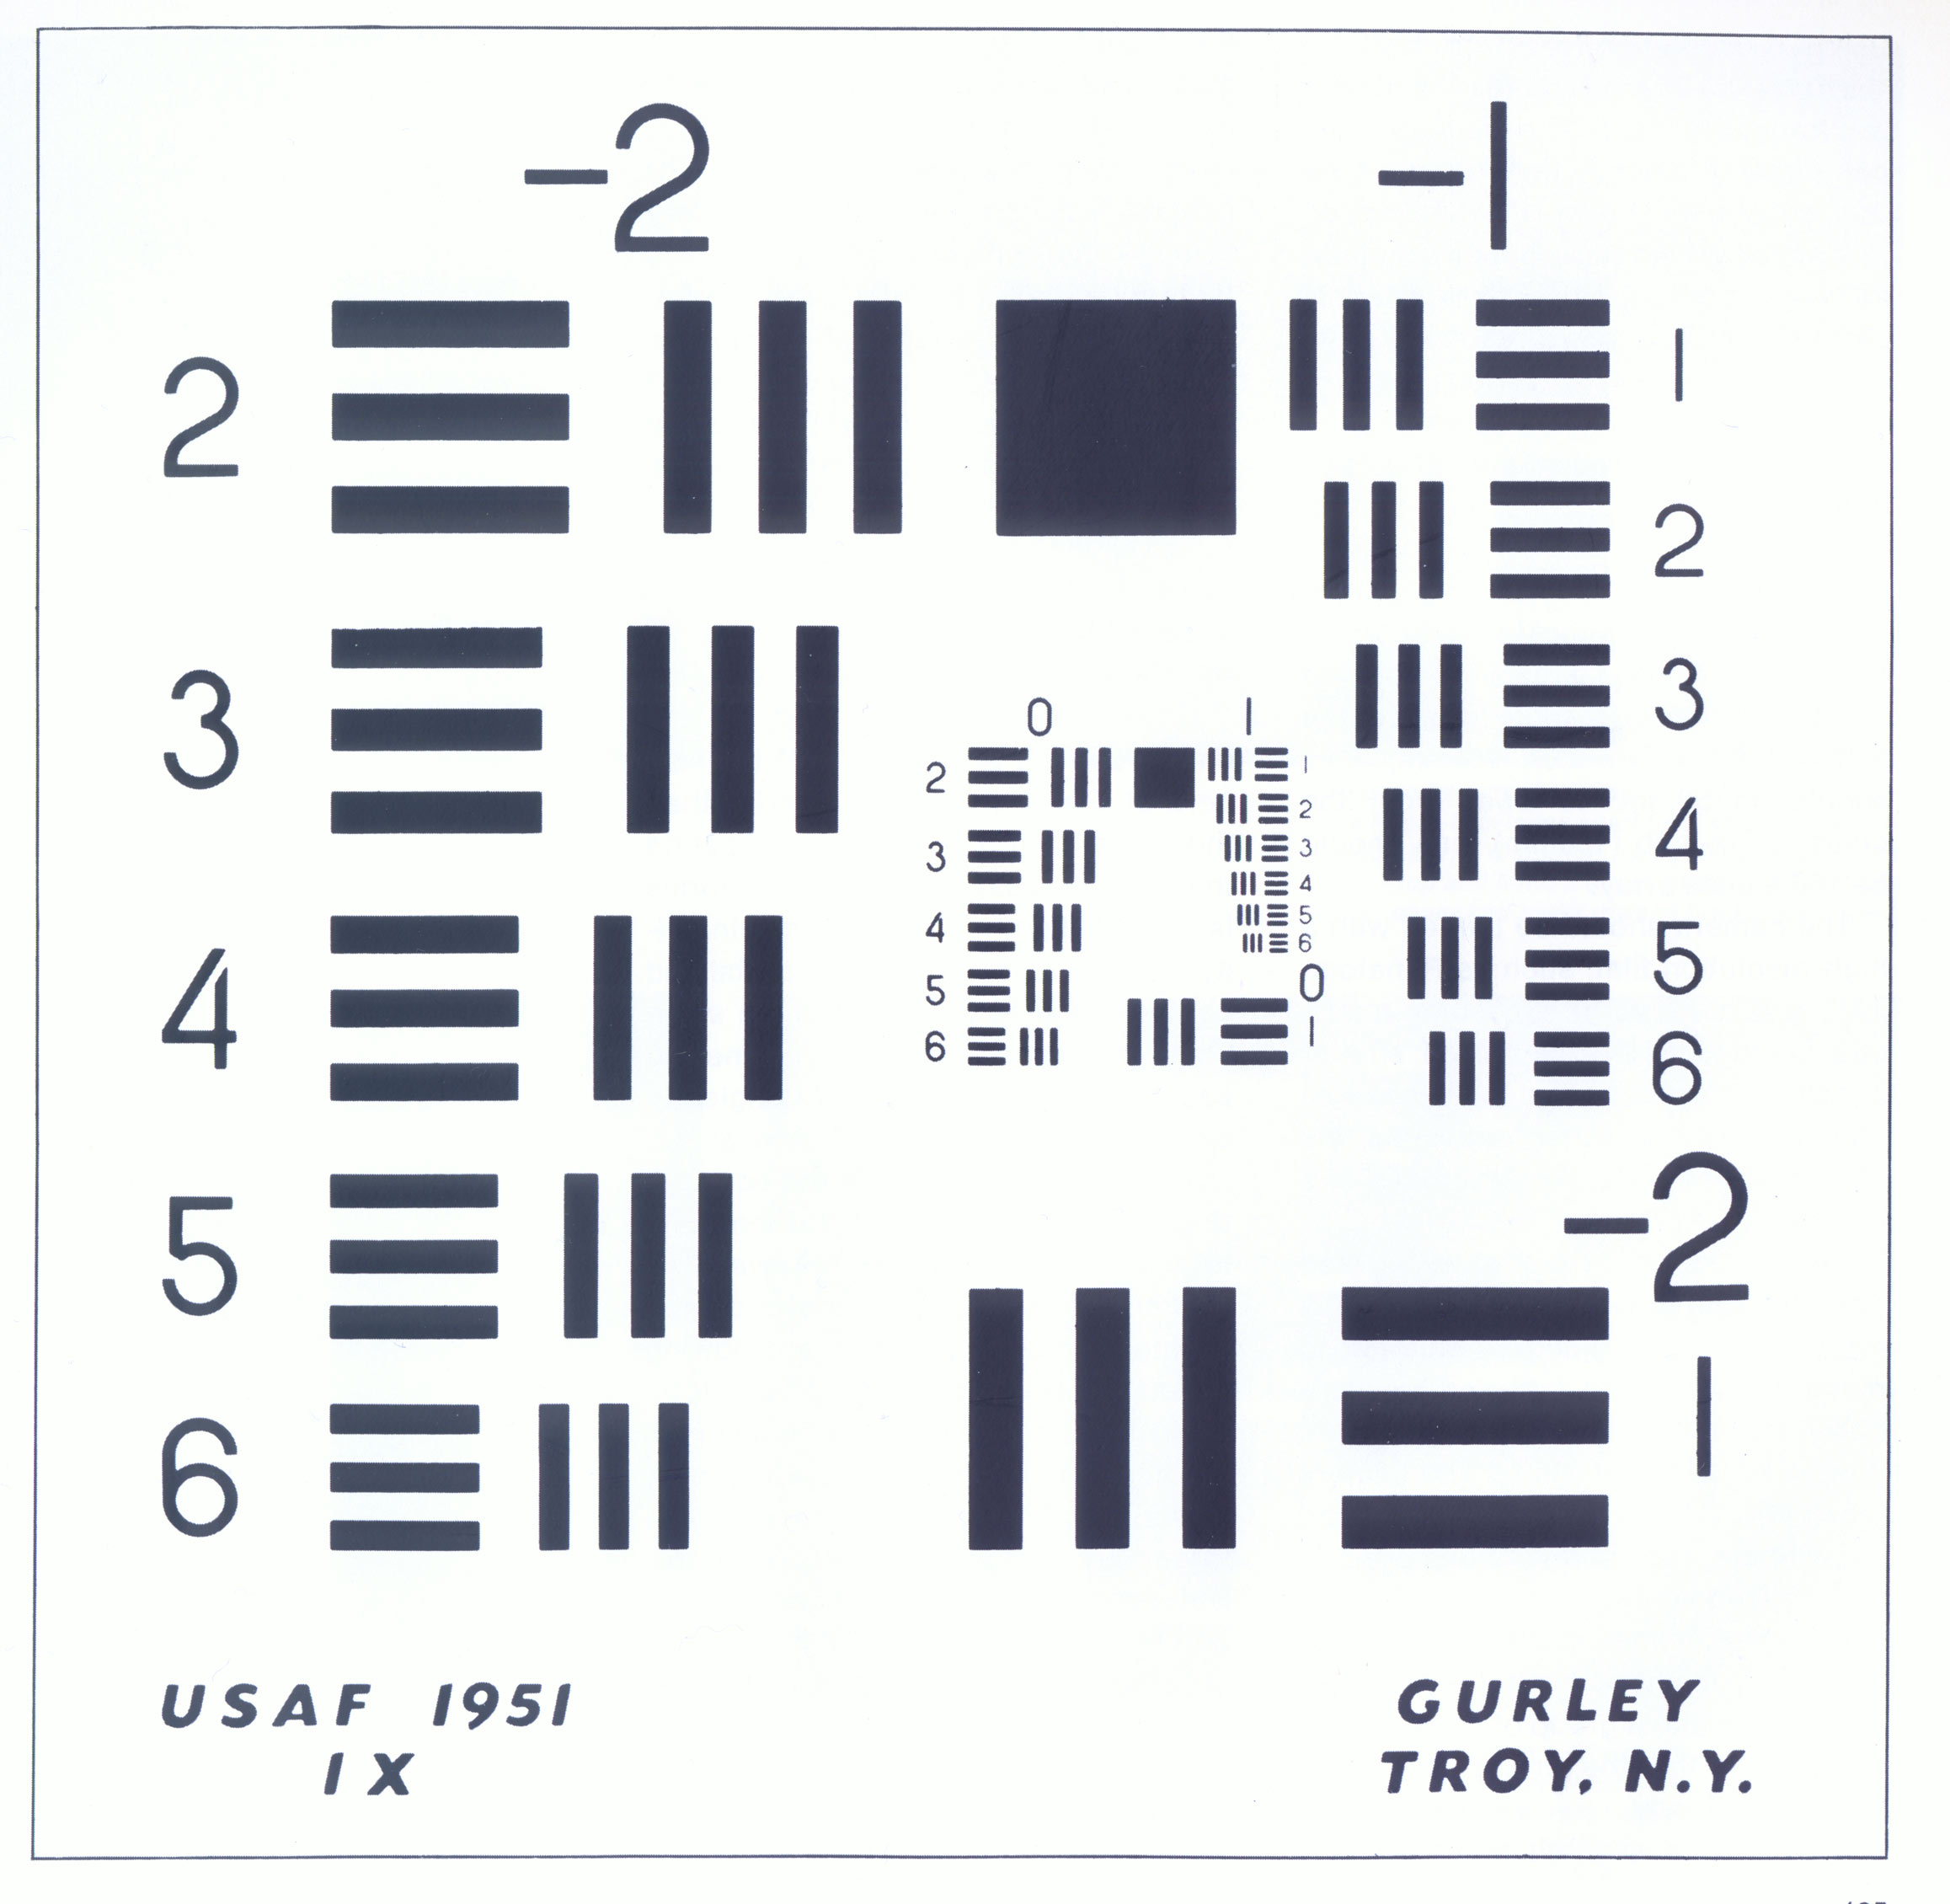
\includegraphics[scale=0.08]{testusaf1951}
	\caption{Test USAF 1951.}\label{fig:usaf1951}
\end{figure}

Posterior a la toma de imágenes, se obtiene a través de estas imágenes un perfil ortogonal a las rendijas de contraste, para cada una de las distintas imágenes. Los resultados se discutirán en la sección~\ref{sec:mtf-directo} del apartado de Resultados experimentales. Este perfil es obtenido mediante un software diseñado en la plataforma de MATLAB que se nos fue otorgado.


\subsection{Medida de la MTF mediante el test de borde (método indirecto)}\label{sec:description:indirecto}

Se obtiene la imagen de la misma manera que el apartado anterior, pero esta vez de una única barra que abarque el campo completo de visión, dividiendo la imagen ortogonalmente como se puede ver en la Fig.~\ref{fig:perfil:img}

De la misma manera se obtiene un perfil de la imagen, por medio del software en MATLAB, los resultados se presentarán en la sección de resultados correspondiente.


\section{Resultados experimentales}\label{sec:resultados}

\subsection{Resultados medidas de la MTF mediante el test de barras (método directo)}\label{sec:mtf-directo}
Se realizó el procedimiento explicado con anterioridad por cada imagen que se obtuvo del test de USAF de referencia. A continuación se presenta algunas de las imágenes estudiadas:

\begin{figure}
\centering
\begin{subfigure}[t]{0.576\textwidth}\centering
	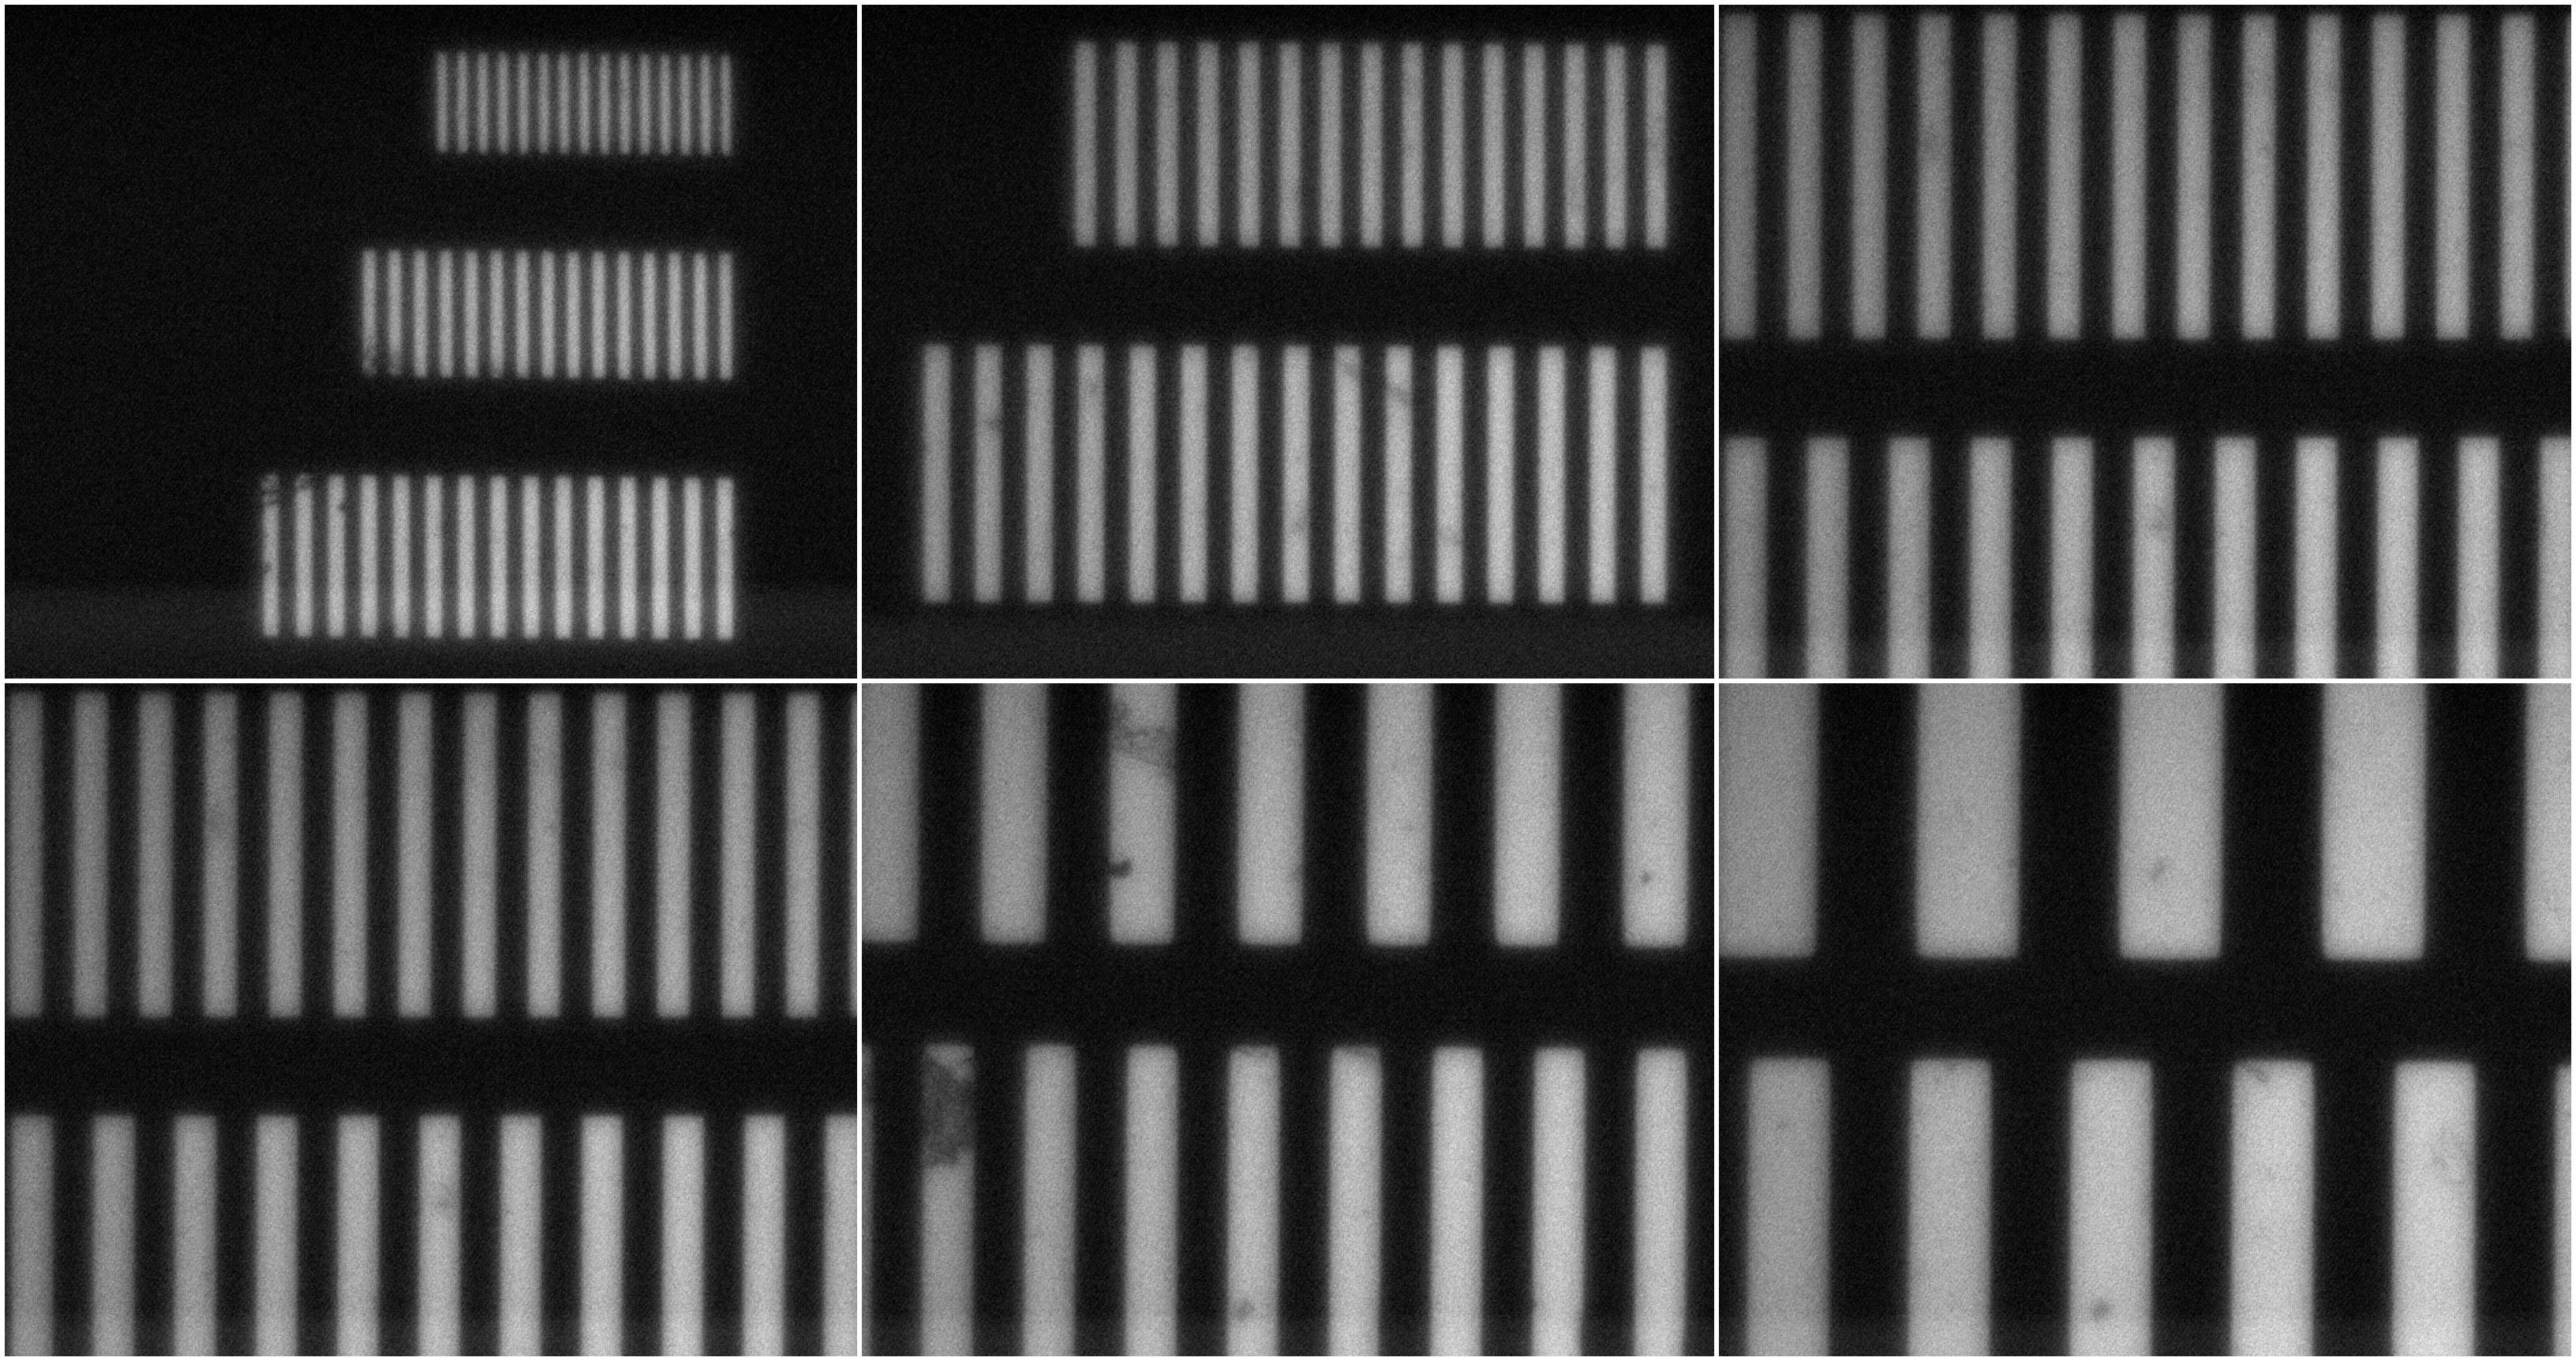
\includegraphics[width=\textwidth]{/imaglineas.jpg}
	\caption{Imágenes tomadas del test de USAF Fig.~\ref{fig:usaf1951} para la medida del MTF directo}\label{fig:images:example}
\end{subfigure}
\,
\begin{subfigure}[t]{0.4\textwidth}\centering
	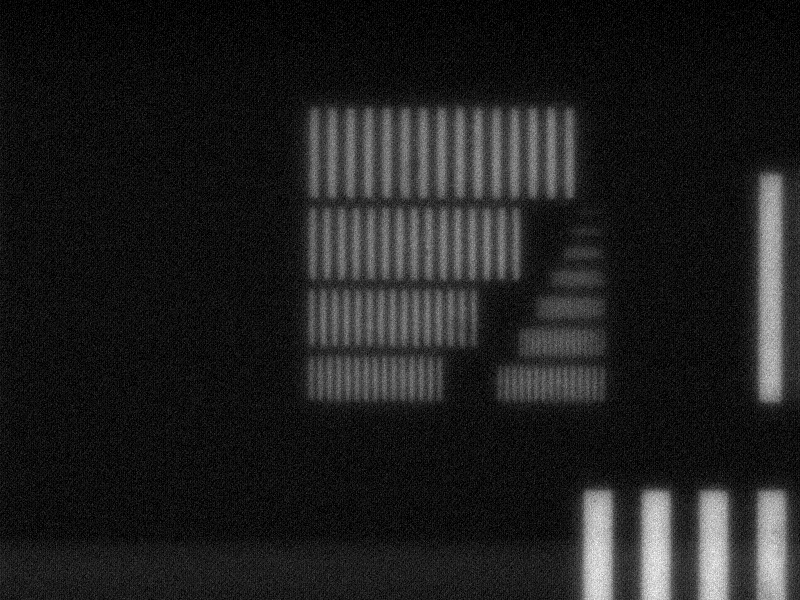
\includegraphics[width=\textwidth]{smallest_lines}
	\caption{Foto tomada durante la práctica de las líneas centrales del test USAF 1951}\label{fig:usafpic}
\end{subfigure}
\caption{Fotos tomadas durante la práctica}\label{fig:group:usaf}
\end{figure}
Procedimiento para sacar el contraste y la frecuencia a partir del perfil de un segmento de líneas: Se obtiene dos posiciones tan distantes como se pueda de dos mínimos de las barras. Se mide la distancia en píxeles entre ellas ($x_{\max} - x_{\min} $), se cuenta el número de periodos entre ellas, que nos permite calcular $T = \flatfrac{(x_{\max} - x_{\min)} }{N_{\textrm{periodos}}}$. A continuación,  se toma los máximos y mínimos de altura $y_{\max}$, $y_{\min}$.

El contraste se ha obtenido a partir de la expresión:
\nopagebreak
\begin{equation}
	C = \frac{y_{\max} - y_{\min}}{y_{\max} + y_{\min}}.
	\label{eq:contraste}
\end{equation}

La frecuencia se calcula como:
\nopagebreak
\begin{equation}
	\nu = \frac{1825}{T}\ \textrm{ciclos/mm},\quad\textrm{TODO: QUE es 1825??}\label{eq:frecuencia}
\end{equation}

Donde el periodo, $T$, se calcula de acuerdo a la gráfica del perfil obtenida en el estudio de cada imagen. Un ejemplo de estas gráficas se muestra en la figura \ref{fig:perfil:example}.

\begin{figure}[!h]
	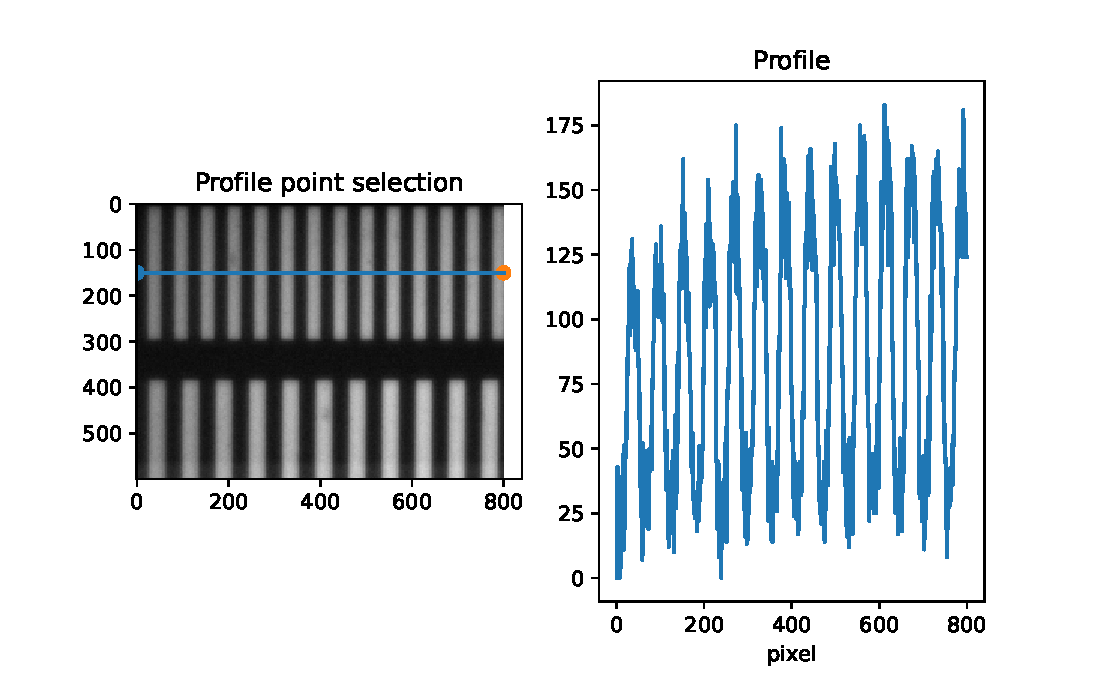
\includegraphics[width=\textwidth]{profile-lines.pdf}
	\caption{Perfil de un segmento de líneas}\label{fig:perfil:example}
\end{figure}


En la tabla \ref{table:perfilintensidad} se recogen medidas tomadas del perfil de intensidad para distintos conjuntos de barras

\begin{table}[hbp]
	\centering
	\csvautotabular[
		table head=\toprule%
		Barras & $y_{\min} (px)$ & $y_{\max} (px)$ & Contraste & $x_{\min} (px)$ & $x_{\max} (px)$ & N Periodos & periodo (px) &  $\flatfrac{\textrm{ciclos}}{\textrm{mm}}$%
		\\\midrule%
	]{practica1/MTF/Profiles.csv}
	\caption{Datos del perfil de intensidad. $y$: intensidad. $x$. El contraste se ha obtenido a partir de la ecuación~\ref{eq:contraste}. La frecuencia se ha obtenido a través de la ecuación~\ref{eq:frecuencia}. Como se obtienen los periodos se explica visualmente en la Fig.~\ref{fig:perfil:example}}%
	\label{table:perfilintensidad}
\end{table}





\subsection{Resultados Medida de la MTF mediante el test de borde (método indirecto)}\label{sec:resultados:indirecto}
Con la imagen del borde obtenida de la imagen patrón USAF de manera que la cámara al tomar la imagen no se encuentre saturada, ingresamos la imagen resultante en el análisis de perfil de intensidad y obtenemos su derivada.

Esto Debido a que la función $\delta(x)$ es la derivada de la step function, $s(x)$, como distribución, podemos usar este hecho para calcular la LSF, encontrando primero la respuesta a un borde, y realizando una estimación de la derivada, podemos obtener la MTF de una manera más rápida.

Se genera la MTF a partir de la LSF y se estima la frecuencia de corte del sistema.

A continuación se muestra los resultados de manera gráfica para mejor interpretación:
\begin{figure}[hptb]
	\centering
	\begin{subfigure}[t]{0.35\textwidth}
		\centering
		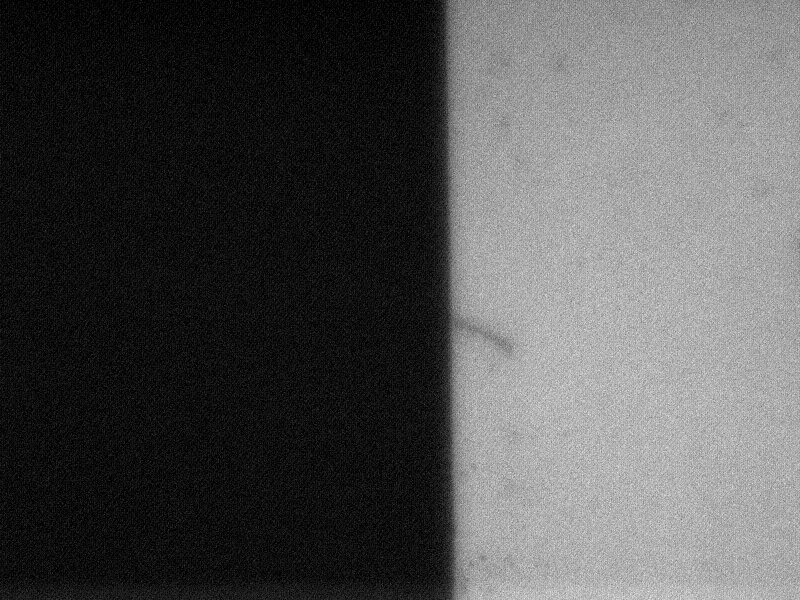
\includegraphics[height=4cm]{edge_large_line}
		\caption{Imagen de una franja amplia}\label{fig:perfil:img}
	\end{subfigure}
	\quad
	\begin{subfigure}[t]{0.60\textwidth}
		\centering
		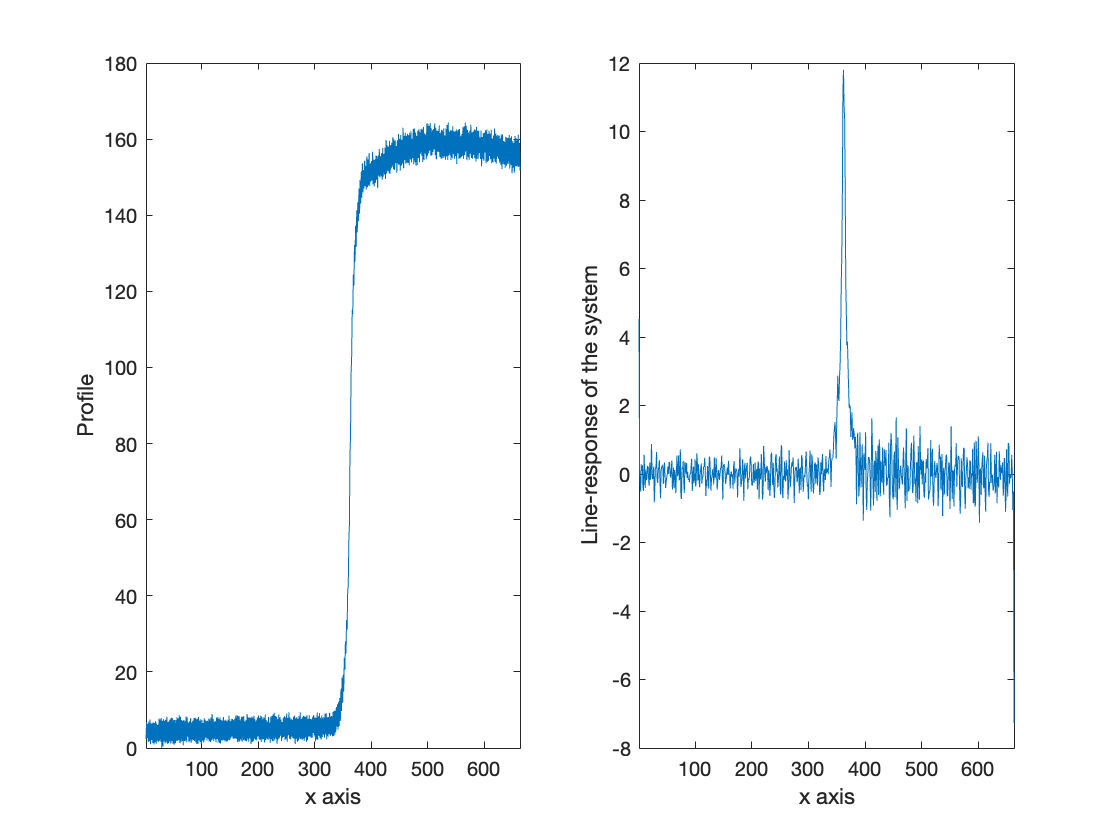
\includegraphics[width=\textwidth, height=4cm]{/lsf_edge.png}
		\caption{Perfil de intensidad de píxeles en una línea horizontal (izqda) y la derivada de este perfil (drcha). La derivada es igual al LSF}\label{fig:perfil:graph}
	\end{subfigure}
	\caption{Perfil de intensidad de una franja grande utilizada para el método indirecto para obtener el MTF, como se describe en la sección~\ref{sec:description:indirecto}}\label{fig:perfil}
\end{figure}

\section{Cuestiones}

\subsection{Sea $H_{c}(u)$ la función de transferencia de un sistema para luz coherente. Escribir la relación entre $H_{c}(u)$ y la función de transferencia del mismo sistema para luz incoherente, $H_{i}(u)$.}\label{sec:cuestion:incoherente}

Cuando la luz incidente es coherente, la imagen resultante se obtiene añadiendo linealmente la amplitud compleja. Sin embargo, cuando la iluminación es idealmente incoherente, la iluminación es linear en la intensidad de la onda incidente. Por ello, en el caso ideal donde la correlación de fase es cero para distintas posiciones, se obtiene que~\cite[p.~132--134]{goodman1996introduction}.
\nopagebreak
\begin{equation}
	I_{i}(u,v) = \kappa \iint_{-\infty}^{\infty}\abs{h(u - \xi, v- \eta)}^{2} I_{g}(\xi, \eta) \dd \xi \dd \eta.
\end{equation}

Por lo tanto, la función $H_{i}(u)$ se puede obtener con el esquema descrito en Fig.~\ref{fig:transformacion}. Básicamente, haciendo la transformación inversa para obtener $h_{c}$, luego multiplicando está con su conjugada, obteniendo $h_{i}$, donde $i$ denota intensidad. Y al realizar la transformada inversa obtenemos el resultado.

\begin{align*}
	H_{i}(u)
	 & = TF\{h_i\}
	= TF\left\{ h_{c} \cdot h^{*}_{c}\right\}
	= TF\left\{ h_{c} \cdot h^{*}_{c}\right\}
	= TF\left\{ TF^{-1}\{H_{c}\} \cdot {TF^{-1}\{H_{c}\}}^{*}\right\}
	\\
	 & = H_{c} \conv H^{*}_{c}. %
	% Numerar sólo la última equación.
	\addtocounter{equation}{1}\tag{\theequation} \label{eq:incoherent-conv}
\end{align*}

\begin{figure}[htpb]
	\begin{center}
		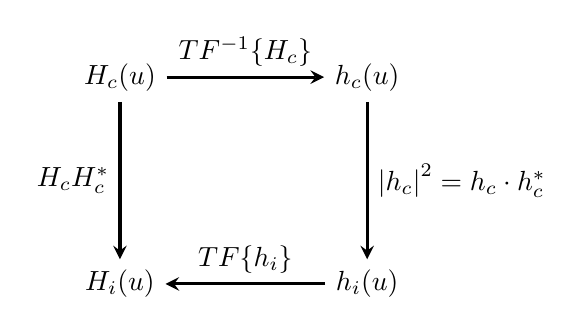
\begin{tikzpicture}[line width=0.4mm, >=stealth]
			\def \n {5}
			\def \radius {3cm}
			\def \margin {8} % margin in angles, depends on the radius

			\node (H) at (0,0) {$H_{c}(u)$};
			\node[right=2cm of H] (h) {$h_{c}(u)$};
			\node[below=2cm of h] (hi) {$h_{i}(u)$};
			\node[below=2cm of H] (Hi) {$H_{i}(u)$};
			\draw[->] (H) -- (h) node[pos=0.5, anchor=south] {$TF^{-1}\{H_{c}\}$};
			\draw[->] (h) -- (hi) node[pos=0.5, anchor=west] {$\abs{h_{c}}^{2} = h_{c} \cdot h^{*}_{c}$};
			\draw[->] (hi) -- (Hi) node[pos=0.5, anchor=south] {$TF\{h_{i}\}$};
			\draw[->] (H) -- (Hi) node[pos=0.5, anchor=east] {$H_{c} \conv H^{*}_{c}$};
		\end{tikzpicture}
	\end{center}
	\caption{Diagrama del proceso para obtener la PTF de intensidad\ref{sec:cuestion:incoherente} }\label{fig:transformacion}
\end{figure}

\subsection{Para un sistema parecido al usado en la práctica:}
	\begin{enumerate}
		\item Estimar la frecuencia de corte de la cámara CCD, $u_{c}^{(CCD)}$, en líneas por milímetro.
		\item Estimar la frecuencia de corte $u_{c}^{(Obj)}$ del objetivo $10\times$ para luz incoherente (la longitud de onda media $\lambda=500\,\unit{\nano\metre}$).
		\item Tomando estos valores y suponiendo que la PSF del objetivo y de la cámara se aproximan por la función $|\sinc(ax)|^2$, dibujar la MTF de cada uno de los elementos y del sistema compuesto.
	\end{enumerate}


\subsection{Aplicar usando el pluging Deconvolutionlab2 y Image J dos métodos de convolución: Regularized Inverse Filter y Richardson-Lucy a una imagen test obtenida por un sistema con una PSF conocida y diferentes tipos de ruido: Gauss y Poisson.}


\begin{figure}[hbp]
	\centering
	\begin{subfigure}[t]{0.45\textwidth}\centering
		\centering
		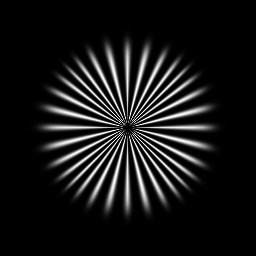
\includegraphics[width=\textwidth]{Simulation deconvolution/ref.jpg}
		\caption{Imagen referencia test original}\label{fig:ref}
	\end{subfigure}
	\hfill
	\begin{subfigure}[t]{0.45\textwidth}\centering
		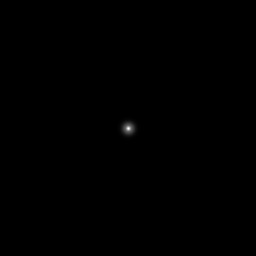
\includegraphics[width=\textwidth]{Simulation deconvolution/psf.jpg}
		\caption{Imagen PSF}\label{fig:psf}
	\end{subfigure}
	\caption{Imagen usada para la simulación con Deconvolutionlab2 y Image J, y el PSF del sistema de captura simulado}\label{fig:image:ref-psf}
\end{figure}
 
 Simulamos tomar fotos de la imagen de referencia (Fig.~\ref{fig:ref}) con un systema con Point Spread Function (PSF) del sistema simulado (Fig.~\ref{fig:psf}). Queremos estudiar distintos tipos de ruido simulado y que algoritmos de de-noising actúan mejor para reducir este ruido.

 Realizamos las siguientes simulaciones de observación con ruido. (Las imágenes obtenidas se ven en Fig.~\ref{fig:convolutions})

\begin{enumerate}
    \item \emph{Noiseless convolution} (convolución sin ruido)
    \item \emph{Simulation with noise-Gauss} (convolución con ruido Gaussiano. $\mu=0$, $\sigma=0.1$, y $0.01$
    \item \emph{Simulation with noise-Poisson} (Convolución con ruido Poisson 0.01, 10 y 0.0001.
    \item Aplicar a las imagenes anteriores \emph{Regularized Inverse filter (RIF)}: =0.01, =1.y Richardson-Lucy (RL) algorithm con 10 y 50 iteraciones. Probamos 100 iteraciones para una caso y comparar con 50 iteraciones
\end{enumerate}

Al realizar el tratado de las imágenes a las cuales se le aplicó ruido, podemos observar a ante la aplicación de un RIF menor con un número de iteraciones menor, se visualiza una recuperación de la imagen mejor filtrada, en cambio, a mayor número de los parámetros anteriormente mencionados la imagen coge más ruido, hasta degradándose en sus colores originales.

Por otro lado, la deconvolución de Richardson-Lucy, al ser procedimiento iterativo para recuperar una imagen subyacente que ha sido añadida ruido por una función de dispersión de puntos conocida, tiene mejores resultados en su filtrado.

\begin{figure}[hbp]
	% Esto no se hace asi con hfill y \, ... pero no me acuerdo como
	\begin{center}
		\,\hfill
		\begin{subfigure}[t]{0.25\textwidth}\centering
			\centering
			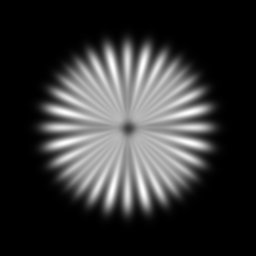
\includegraphics[width=\textwidth]{Simulation deconvolution/ref_conv}
			\caption{Convolution noiseless}\label{fig:sim:conv}
		\end{subfigure}
		\,\hfill
		\begin{subfigure}[t]{0.25\textwidth}\centering
			\centering
			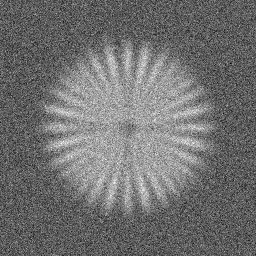
\includegraphics[width=\textwidth]{Simulation deconvolution/ref_ng_0.1}
			\caption{Convolution NG. $Mean=0$, $Stdev=0.1$}\label{fig:sim:ng0.1}
		\end{subfigure}
		\hfill
		\begin{subfigure}[t]{0.25\textwidth}\centering
			\centering
			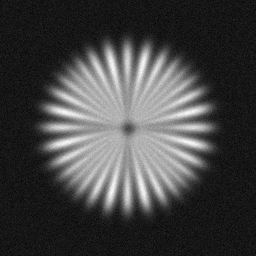
\includegraphics[width=\textwidth]{Simulation deconvolution/ref_ng_0.01}
			\caption{Convolution NG. $Mean=0$, $Stdev=0.01s$}\label{fig:sim:ng0.01}
		\end{subfigure}
		\hfill\,
		\\
		\hfill\,
		\begin{subfigure}[t]{0.25\textwidth}\centering
			\centering
			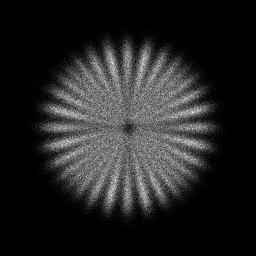
\includegraphics[width=\textwidth]{Simulation deconvolution/ref_np_0.01}
			\caption{Convolution NP 0.01}\label{fig:sim:np0.01}
		\end{subfigure}
		\hfill
		\begin{subfigure}[t]{0.25\textwidth}\centering
			\centering
			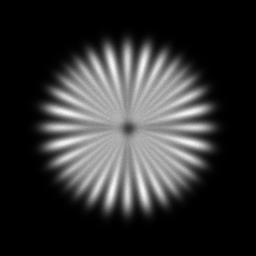
\includegraphics[width=\textwidth]{Simulation deconvolution/ref_np_0.0001}
			\caption{Convolution NP 0.0001}
		\end{subfigure}
		\hfill
		\begin{subfigure}[t]{0.25\textwidth}\centering
			\centering
			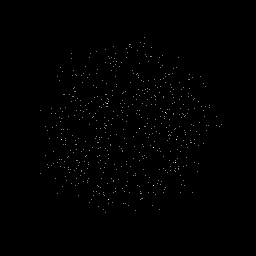
\includegraphics[width=\textwidth]{Simulation deconvolution/ref_np_10}
			\caption{Convolution NP 10}
		\end{subfigure}
		\hfill\,
		\caption{Simulación de la figura ~\ref{fig:image:ref-psf} con distintos tipos de ruido}\label{fig:convolutions}
	\end{center}
\end{figure}


\begin{figure}[hbp]
	\centering
	\begin{tabular}[t]{l c c c c}
		Original Image                                                                  & RIF 0.01 & RIF 1 & RL 10 & RL 50 \\
		Fig.~\ref{fig:sim:conv}                                                         &
		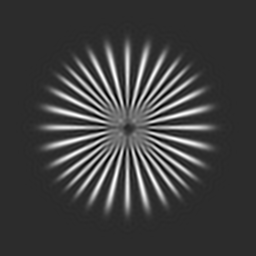
\includegraphics[scale=0.25]{Simulation deconvolution/ref_conv/RIF_0.01.png}    &
		
\includegraphics[scale=0.25]{Simulation deconvolution/ref_conv/RIF_1.png}       &
		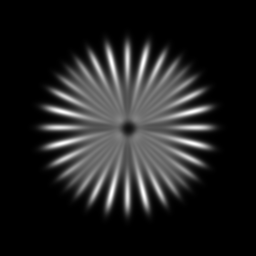
\includegraphics[scale=0.25]{Simulation deconvolution/ref_conv/RL_10.png}       &
		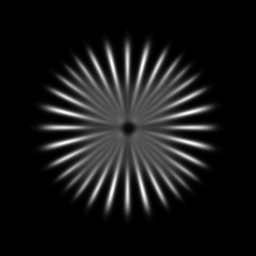
\includegraphics[scale=0.25]{Simulation deconvolution/ref_conv/RL_50.png}
		\\
		Fig.~\ref{fig:sim:ng0.1}                                                        &
		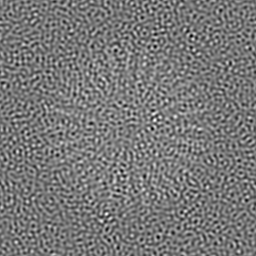
\includegraphics[scale=0.25]{Simulation deconvolution/ref_ng_0.1/RIF_0.01.png}  &
		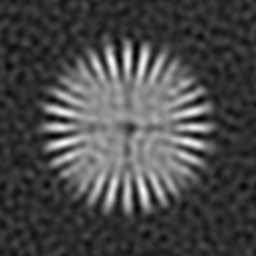
\includegraphics[scale=0.25]{Simulation deconvolution/ref_ng_0.1/RIF_1.png}     &
		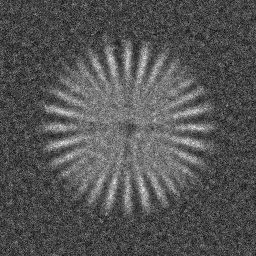
\includegraphics[scale=0.25]{Simulation deconvolution/ref_ng_0.1/RL_10.png}     &
		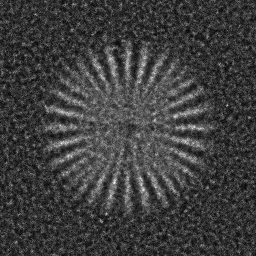
\includegraphics[scale=0.25]{Simulation deconvolution/ref_ng_0.1/RL_50.png}
		\\
		Fig.~\ref{fig:sim:ng0.01}                                                       &
		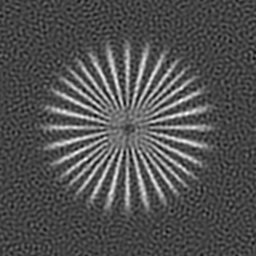
\includegraphics[scale=0.25]{Simulation deconvolution/ref_ng_0.01/RIF_0.01.png} &
		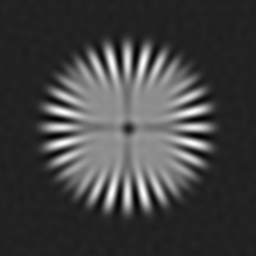
\includegraphics[scale=0.25]{Simulation deconvolution/ref_ng_0.01/RIF_1.png}    &
		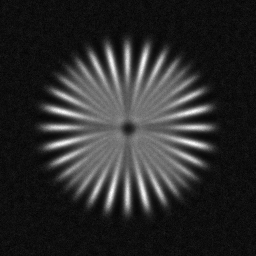
\includegraphics[scale=0.25]{Simulation deconvolution/ref_ng_0.01/RL_10.png}    &
		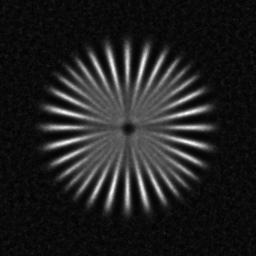
\includegraphics[scale=0.25]{Simulation deconvolution/ref_ng_0.01/RL_50.png}
		\\
		Fig.~\ref{fig:sim:np0.01}                                                       &
		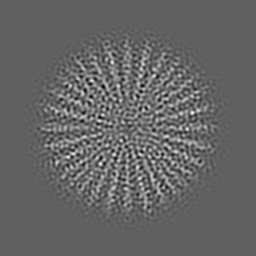
\includegraphics[scale=0.25]{Simulation deconvolution/ref_np_0.01/RIF_0.01.png} &
		
\includegraphics[scale=0.25]{Simulation deconvolution/ref_np_0.01/RIF_1.png}    &
		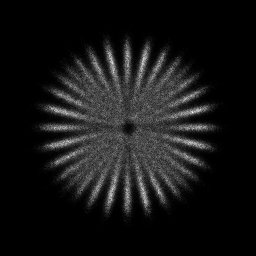
\includegraphics[scale=0.25]{Simulation deconvolution/ref_np_0.01/RL_10.png}    &
		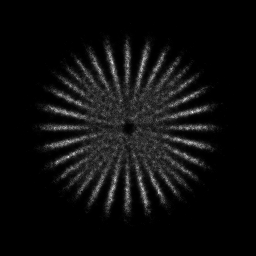
\includegraphics[scale=0.25]{Simulation deconvolution/ref_np_0.01/RL_50.png}
		\\
	\end{tabular}
	\caption{Matriz de los filtros realizados para recuperar las imágenes con ruido añadido simulado. Cada fila d se corresponde a una figura de \ref{fig:convolutions} (a--d), cada columna indica un método de recuperación}
\end{figure}

%%%%%%%%%% If using BibTeX:
\bibliography{bibliography}

\end{document}
